% !Rnw root = ../mlcrash.Rnw




%%%%%%%%%%%%%%%%%%%%%%%%%%%%
\part{Opening the Black Box}
%%%%%%%%%%%%%%%%%%%%%%%%%%%%

\newthought{It's now time to see some of this in action}.  In the following will will try a variety of techniques so as to get a better feel for the sorts of things we might try out.

\section{The Dataset}
We will use the wine data set from the UCI Machine Learning data repository.  The goal is to predict wine quality, of which there are 7 values (integers 3-9).  We will turn this into a binary classification task to predict whether a wine is 'good' or not, which is arbitrarily chosen as 6 or higher.  After getting the hang of things one might redo the analysis as a multiclass problem or even toy with regression approaches, just note there are very few 3s or 9s so you really only have 5 values to work with.  The original data along with detailed description can be found \href{http://archive.ics.uci.edu/ml/datasets/Wine+Quality}{here}, but aside from quality it contains predictors such as residual sugar, alcohol content, acidity and other characteristics of the wine\sidenote{I think it would be interesting to have included characteristics of the people giving the rating.}.

The original data is separated into white and red data sets. I have combined them and created additional variables: \emph{color} and its numeric version \emph{white} indicating white or red, and \emph{good}, indicating scores greater than 7 (denoted as 'Yes').  The following will show some basic numeric information about the data.

\begin{knitrout}\footnotesize
\definecolor{shadecolor}{rgb}{0.969, 0.969, 0.969}\color{fgcolor}\begin{kframe}
\begin{alltt}
wine = \hlfunctioncall{read.csv}(\hlstring{"http://www.nd.edu/~mclark19/learn/data/goodwine.csv"})
\hlfunctioncall{summary}(wine)
\end{alltt}
\begin{verbatim}
##  fixed.acidity   volatile.acidity  citric.acid    residual.sugar 
##  Min.   : 3.80   Min.   :0.08     Min.   :0.000   Min.   : 0.60  
##  1st Qu.: 6.40   1st Qu.:0.23     1st Qu.:0.250   1st Qu.: 1.80  
##  Median : 7.00   Median :0.29     Median :0.310   Median : 3.00  
##  Mean   : 7.21   Mean   :0.34     Mean   :0.319   Mean   : 5.44  
##  3rd Qu.: 7.70   3rd Qu.:0.40     3rd Qu.:0.390   3rd Qu.: 8.10  
##  Max.   :15.90   Max.   :1.58     Max.   :1.660   Max.   :65.80  
##    chlorides     free.sulfur.dioxide total.sulfur.dioxide    density     
##  Min.   :0.009   Min.   :  1.0       Min.   :  6          Min.   :0.987  
##  1st Qu.:0.038   1st Qu.: 17.0       1st Qu.: 77          1st Qu.:0.992  
##  Median :0.047   Median : 29.0       Median :118          Median :0.995  
##  Mean   :0.056   Mean   : 30.5       Mean   :116          Mean   :0.995  
##  3rd Qu.:0.065   3rd Qu.: 41.0       3rd Qu.:156          3rd Qu.:0.997  
##  Max.   :0.611   Max.   :289.0       Max.   :440          Max.   :1.039  
##        pH         sulphates        alcohol        quality       color     
##  Min.   :2.72   Min.   :0.220   Min.   : 8.0   Min.   :3.00   red  :1599  
##  1st Qu.:3.11   1st Qu.:0.430   1st Qu.: 9.5   1st Qu.:5.00   white:4898  
##  Median :3.21   Median :0.510   Median :10.3   Median :6.00               
##  Mean   :3.22   Mean   :0.531   Mean   :10.5   Mean   :5.82               
##  3rd Qu.:3.32   3rd Qu.:0.600   3rd Qu.:11.3   3rd Qu.:6.00               
##  Max.   :4.01   Max.   :2.000   Max.   :14.9   Max.   :9.00               
##      white        good     
##  Min.   :0.000   No :2384  
##  1st Qu.:1.000   Yes:4113  
##  Median :1.000             
##  Mean   :0.754             
##  3rd Qu.:1.000             
##  Max.   :1.000
\end{verbatim}
\end{kframe}
\end{knitrout}



\section{R Implementation}
I will use the \textcolor{blue}{caret} package in R.  Caret makes implementation of validation, data partitioning, performance assessment, and prediction and other procedures about as easy as it can be in this environment.  However, caret is using other R packages that have more information about the specific functions underlying the process.  Check out the \href{http://caret.r-forge.r-project.org/}{caret home page} for more detail.

\section{Feature Selection \& The Data Partition}
This data set is large enough to leave a holdout sample, allowing us to initially search for the best of a given modeling approach over a grid of tuning parameters specific to the technique.  To iterate previous discussion, we don't want test performance contaminated with the tuning process.  With the best model at $t$ tuning parameter(s), we will assess performance with prediction on the holdout set.

\marginnote{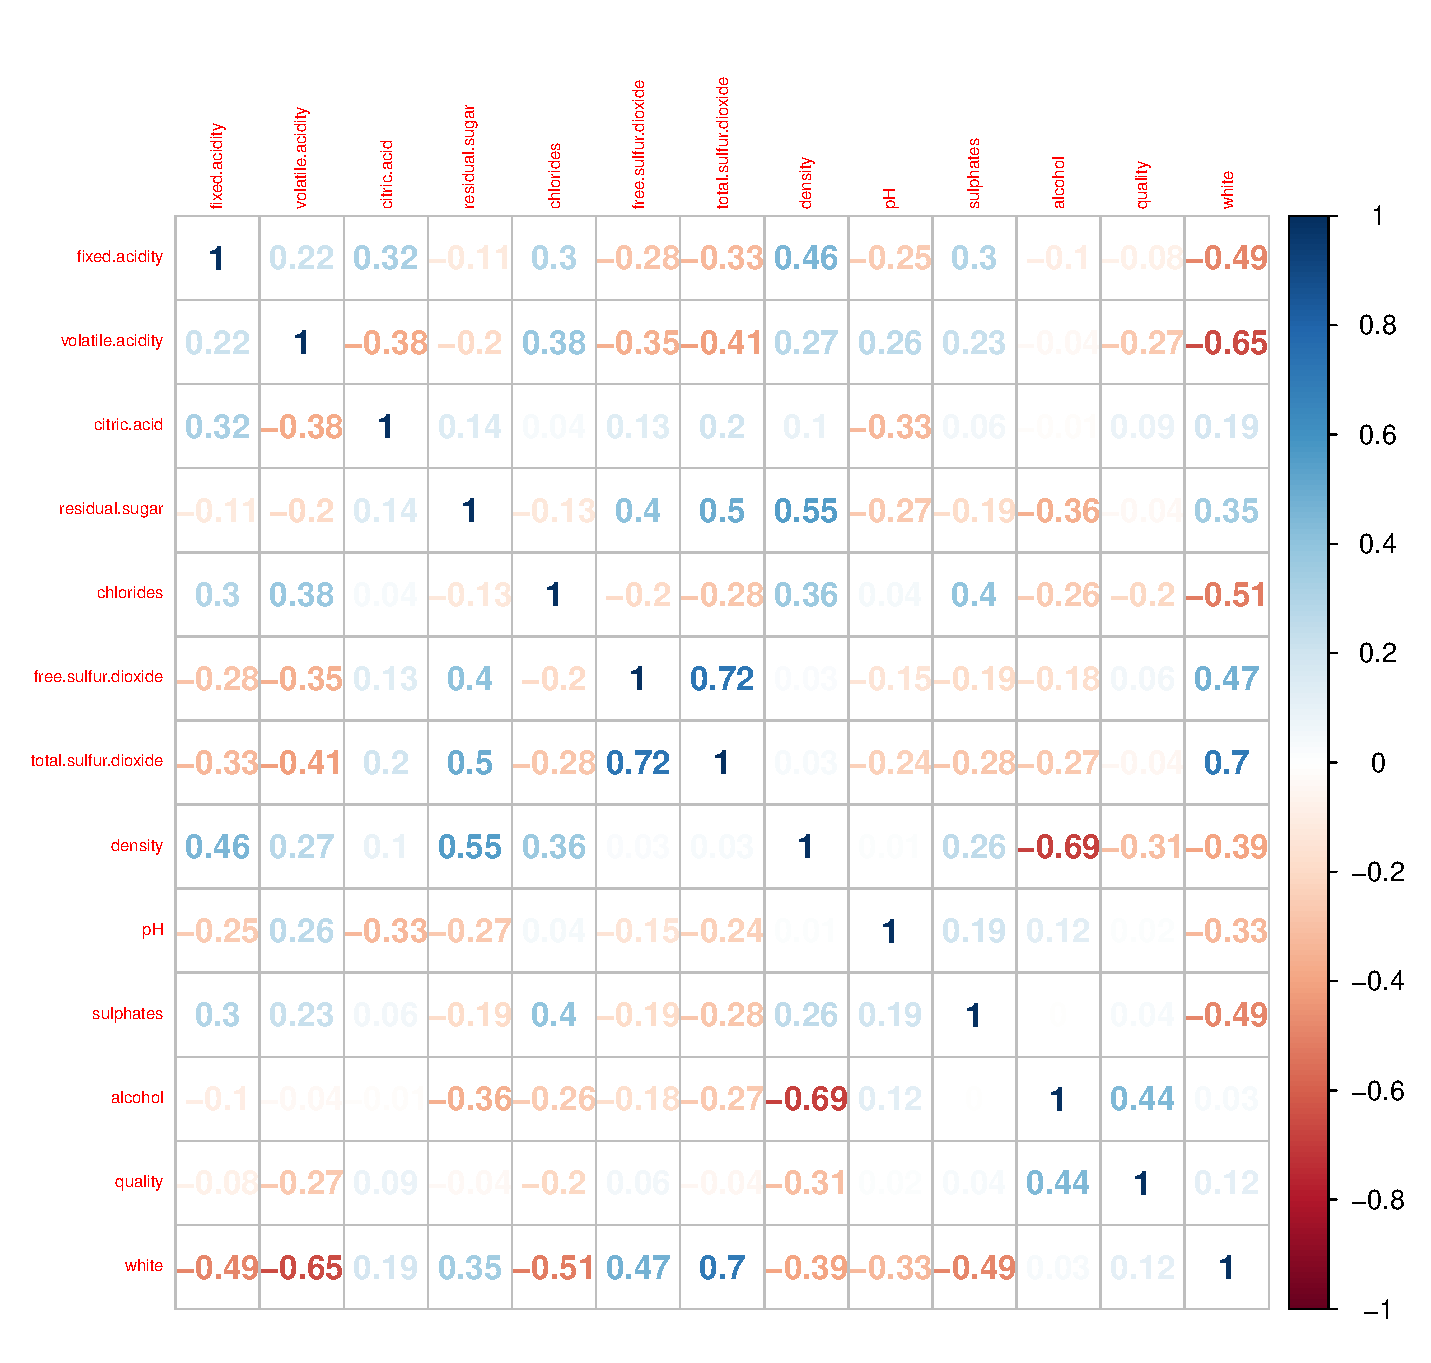
\includegraphics[scale=.25]{images/corrplot}}
I also made some decisions to deal with the notable collinearity in the data, which can severely hamper some methods.  We can look at the simple correlation matrix to start

\begin{knitrout}\footnotesize
\definecolor{shadecolor}{rgb}{0.969, 0.969, 0.969}\color{fgcolor}\begin{kframe}
\begin{alltt}
\hlfunctioncall{library}(corrplot)
\hlfunctioncall{corrplot}(\hlfunctioncall{cor}(wine[, -\hlfunctioncall{c}(13, 15)]), method = \hlstring{"number"}, tl.cex = 0.5)
\end{alltt}
\end{kframe}
\end{knitrout}


I ran regressions to examine the r-squared for each predictor in a model as if it were the dependent variable predicted by the other input variables.  The highest was for density at over 96\%, and further investigation suggested color and either sulfur dioxide are largely captured by the other variables already also.  These will not be considered in the following models.

Caret has its own partitioning function we can use here to separate the data into training and test data.  There are 6497 records of which I will put 80\% into the training set.  The function \textcolor{red}{createDataPartition} will produce indices to use as the training set.  In addition to this, we will normalize the continuous variables to the [0,1] range.

\begin{knitrout}\footnotesize
\definecolor{shadecolor}{rgb}{0.969, 0.969, 0.969}\color{fgcolor}\begin{kframe}
\begin{alltt}
\hlfunctioncall{library}(caret)
\hlfunctioncall{set.seed}(1234)  \hlcomment{#so that the indices will be the same when re-run}
trainIndices = \hlfunctioncall{createDataPartition}(wine$good, p = 0.8, list = F)
wine_train = wine[trainIndices, -\hlfunctioncall{c}(6, 8, 12:14)]  \hlcomment{#remove quality and color, as well as density and others}
prep_train = \hlfunctioncall{preProcess}(wine_train[, -10], method = \hlstring{"range"})  # omit target
wine_train = \hlfunctioncall{data.frame}(\hlfunctioncall{predict}(prep_train, wine_train[, -10]), good = wine_train[, 
    10])

wine_test = wine[!1:\hlfunctioncall{nrow}(wine) %in% trainIndices, -\hlfunctioncall{c}(6, 8, 12:14)]
prep_test = \hlfunctioncall{preProcess}(wine_test[, -10], method = \hlstring{"range"})
wine_test = \hlfunctioncall{data.frame}(\hlfunctioncall{predict}(prep_test, wine_test[, -10]), good = wine_test[, 
    10])
\end{alltt}
\end{kframe}
\end{knitrout}


\marginnote{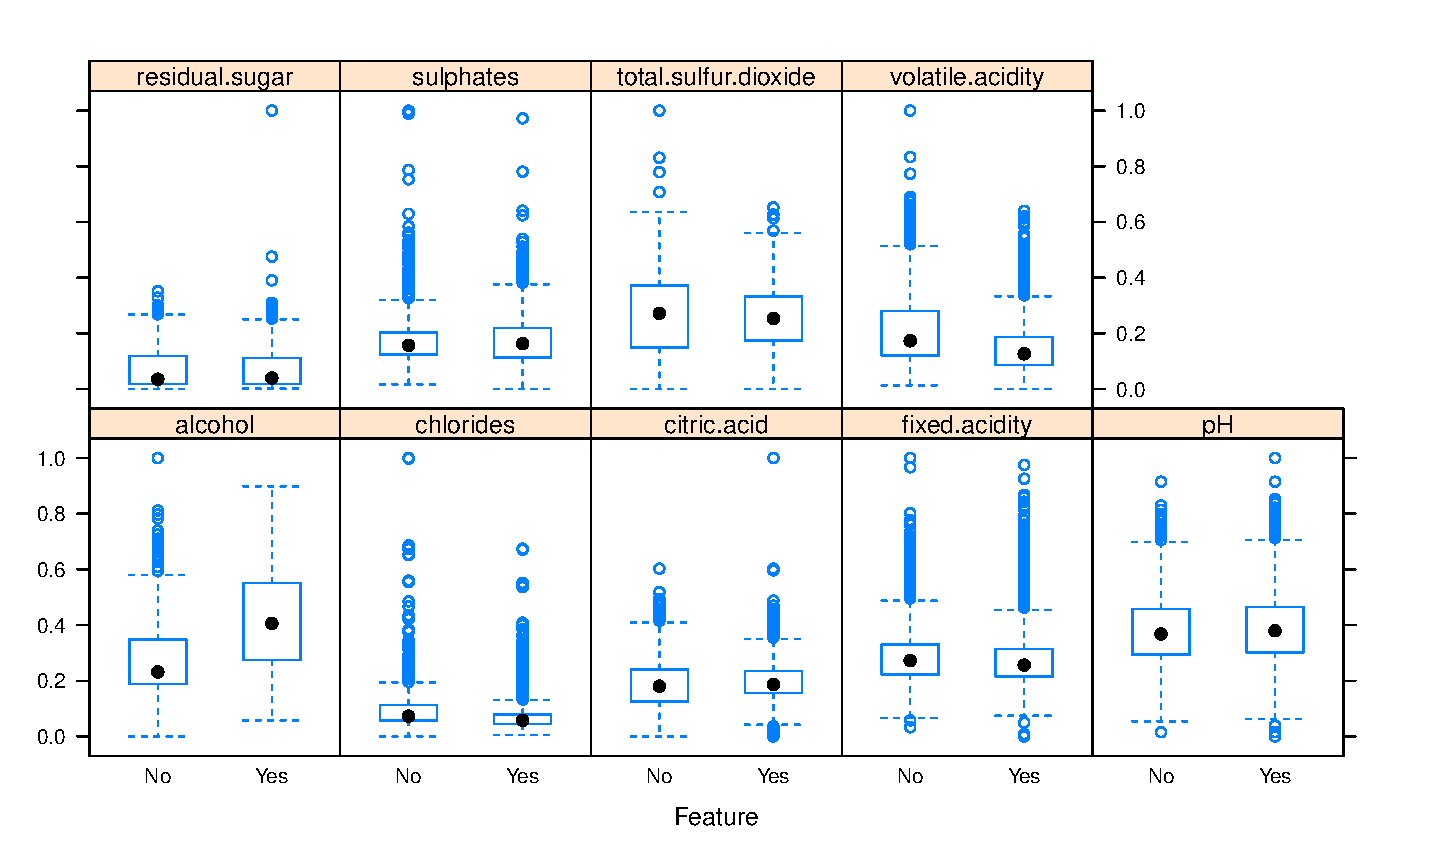
\includegraphics[scale=.25]{images/classbox}}
Let's take an initial peek at how the predictors separate on the target.  

\begin{knitrout}\footnotesize
\definecolor{shadecolor}{rgb}{0.969, 0.969, 0.969}\color{fgcolor}\begin{kframe}
\begin{alltt}
\hlfunctioncall{featurePlot}(wine_train[, -10], wine_train$good, \hlstring{"box"})
\end{alltt}
\end{kframe}
\end{knitrout}


For the training set, it looks like alcohol content, volatile acidity and chlorides separate most with regard to good classification. While this might give us some food for thought, note that the figure does not give insight into interaction effects, which methods such as trees will get at.

%%%
\section{$k$-nearest Neighbors}
Consider the typical distance matrix\sidenote{See, for example, the function \textcolor{red}{dist} in R.} that is often used for cluster analysis of observations\sidenote{Often referred to as \emph{unsupervised} learning as there is not target/dependent variable.}. If we choose something like \emph{Euclidian distance} as a metric, each point in the matrix gives the value of how far an observation is from some other, given their respective values on a set of variables.

K-nearest neighbors approaches exploit this information for predictive purposes.  Let us take a classification example, and $k = 5$ neighbors.  For a given observation $x_i$, find the 5 closest $k$ neighbors in terms of Euclidean distance based on the predictor variables.  The class that is predicted is whatever class the majority of the neighbors are labeled as\sidenote{See the \textcolor{red}{knn.ani} function in the \textcolor{blue}{animation} package for a visual demonstration}.  For continuous outcomes we might take the mean of those neighbors as the prediction.

So how many neighbors would work best? This is an example of a tuning parameter, i.e. $k$, for which we have no knowledge about its value without doing some initial digging.  As such we will select the tuning parameter as part of the validation process.

The caret package provides several techniques for validation such as $k$-fold, bootstrap, leave-one-out and others.  We will use 10-fold crossvalidation.  We will also set up a set of values for k to try out\sidenote{For whatever tuning parameters are sought, the train function will expect a dataframe with a '.' before the parameter name as the column name.  Note also you can just specify a tuning length instead.  See the help file for the \textcolor{red}{train} function.}.



















